\documentclass[math-font=newcm]{sjtuarticle}
\allowdisplaybreaks
\usepackage[style=gb7714-2015]{biblatex}
\addbibresource{ref.bib}
\usepackage{subcaption}
\usepackage{ntheorem}
\usepackage{tikz}
\usetikzlibrary{3d,perspective}
\usepackage{forest}
\usepackage[colorlinks]{hyperref}

\title{作业3}
\author{李子龙\\123033910195}
\begin{document}
\maketitle

\tableofcontents*
% \clearpage

\section{第1题}

Prove that two successive 2D rotations are additive:
\begin{equation}
    R(\theta_1) R(\theta_2) = R(\theta_1 + \theta_2) 
\end{equation}

\begin{proof}
    根据二维旋转的定义有
    \begin{align*}
        R(\theta_1)R(\theta_2)&=\begin{pmatrix}
            \cos\theta_1 & -\sin\theta_1 \\
            \sin\theta_1 & \cos\theta_1
        \end{pmatrix}\begin{pmatrix}
            \cos\theta_2 & -\sin\theta_2 \\
            \sin\theta_2 & \cos\theta_2
        \end{pmatrix} \\
        &=\begin{pmatrix}
            \cos\theta_1\cos\theta_2-\sin\theta_1\sin\theta_2 &
            -\cos\theta_1\sin\theta_2-\sin\theta_1\cos\theta_2 \\
            \sin\theta_1\cos\theta_2+\cos\theta_1\sin\theta_2 &
            -\sin\theta_1\sin\theta_2+\cos\theta_1\cos\theta_2
        \end{pmatrix} \\
        &=\begin{pmatrix}
            \cos(\theta_1+\theta_2) & -\sin(\theta_1+\theta_2) \\
            \sin(\theta_1+\theta_2) & \cos(\theta_1+\theta_2)
        \end{pmatrix}\\
        &=R(\theta_1+\theta_2)
    \end{align*}
    即二维旋转是加性的。
\end{proof}

\section{第2题}

Consider a line from the origin of a right-handed coordinate system to the point $P(x, y, z)$. Find the transformation matrices needed to rotate the line into the positive $z$ axis in two different ways, and show by algebraic
manipulation that, in each case, the point $P$ does go to the $z$ axis. For each method, calculate the sines and
cosines of the angles of rotation.
\begin{enumerate}
    \item[a.] Rotate about the $y$ axis into the $(y, z)$plane, then rotate about the $x$ axis into the $z$ axis.
    \item[b.] Rotate about the $z$ axis into the $(x, z)$plane, then rotate about the $y$ axis into the $z$ axis.
\end{enumerate}

\begin{solution}
    \begin{figure}[h]
        \begin{subfigure}{.5\textwidth}
        \centering
        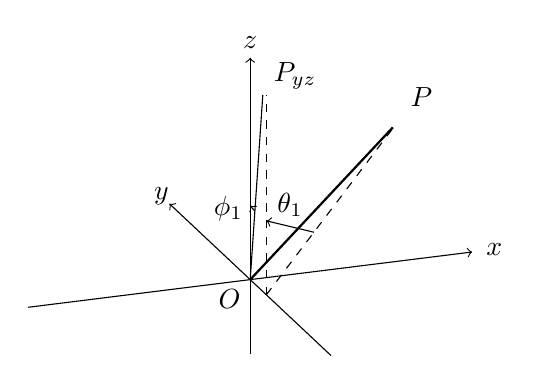
\begin{tikzpicture}[]
            \begin{scope}[3d view={-20}{20}]
              \draw[->] (-3,0,0) -- (3,0,0) node[pos=1.05]{$x$};
              \draw[->] (0,-3,0) -- (0,3,0) node[pos=1.05]{$y$};
              \draw[->] (0,0,-1) -- (0,0,3) node[pos=1.05]{$z$};
              \node [below left] at (0,0,0) {$O$};
              \pgfmathsetmacro\az{50}
            %   \begin{scope}[canvas is xy plane at z=0]
                % \draw[->] (0,0) ++(0,-2) arc (-90:-90+\az:2) coordinate[pos=0.5](az);
                % \draw (az) -- ++(-90+\az/2:1) node[below]{$\theta$};
                % \draw[thick,dashed] (0,0) -- ++(-90+\az:3);
            %   \end{scope}
              \begin{scope}[canvas is xz plane at y=-0.6]
                \draw[dashed] (0,0) --++ (\az:2.7);
                \draw[dashed] (0,0) --++ (90:2.7);
                \draw[->] (\az:1) --node[above]{$\theta_1$} (90:1);
              \end{scope}
              \begin{scope}[canvas is yz plane at x=0]
                \draw (0,0) --node[right,pos=1.1]{$P_{yz}$}++ (100:2.7);
                \draw[->] (100:1) --node[left]{$\phi_1$}(90:1);
              \end{scope}
              \begin{scope}[rotate around z=\az]
                \pgfmathsetmacro\el{50}
                \begin{scope}[canvas is yz plane at x=0]
                %   \draw[->] (0,0) ++(-2.5,0) arc (180:180-\el:2.5) coordinate[pos=0.5](el);
                %   \draw (el) -- ++(180-\el/2:1) node[above]{$\phi$};
                  \draw[thick] (0,0) -- node[pos=1.2] {$P$} ++(180-\el:3);
                \end{scope}
              \end{scope}
            \end{scope}
          \end{tikzpicture}
          \caption{先绕$y$轴旋转,再绕$x$轴旋转}
          \label{fig:a}
        \end{subfigure}
        \begin{subfigure}{.5\textwidth}
            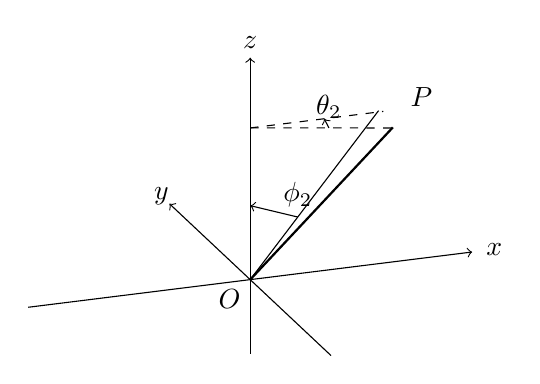
\begin{tikzpicture}[]
                \begin{scope}[3d view={-20}{20}]
                  \draw[->] (-3,0,0) -- (3,0,0) node[pos=1.05]{$x$};
                  \draw[->] (0,-3,0) -- (0,3,0) node[pos=1.05]{$y$};
                  \draw[->] (0,0,-1) -- (0,0,3) node[pos=1.05]{$z$};
                  \node [below left] at (0,0,0) {$O$};
                  \pgfmathsetmacro\az{50}
                %   \begin{scope}[canvas is xy plane at z=0]
                    % \draw[->] (0,0) ++(0,-2) arc (-90:-90+\az:2) coordinate[pos=0.5](az);
                    % \draw (az) -- ++(-90+\az/2:1) node[below]{$\theta$};
                    % \draw[thick,dashed] (0,0) -- ++(-90+\az:3);
                %   \end{scope}
                %   \begin{scope}[canvas is xz plane at y=-0.6]
                %     \draw[dashed] (0,0) --++ (\az:2.7);
                %     \draw[dashed] (0,0) --++ (90:2.7);
                %     \draw[->] (\az:1) --node[above]{$\theta_1$} (90:1);
                %   \end{scope}
                %   \begin{scope}[canvas is yz plane at x=0]
                %     \draw (0,0) --node[right,pos=1.1]{$P_{yz}$}++ (100:2.7);
                %     \draw[->] (100:1) --node[left]{$\phi_1$}(90:1);
                %   \end{scope}
                \begin{scope}[canvas is xz plane at y=0]
                    \draw (0,0) --++ (\az:2.7);
                    \draw[->] (\az:1) node[above] {$\phi_2$} -- (90:1);
                \end{scope}
                \begin{scope}[canvas is xy plane at z=2.05]
                    \draw[dashed] (0,0) --++ (-20:1.8);
                    \draw[dashed] (0,0) --++ (0:1.8);
                    \draw[->] (-20:1) node[above] {$\theta_2$} --(0:1);
                \end{scope}
                \begin{scope}[rotate around z=\az]
                    \pgfmathsetmacro\el{50}
                    \begin{scope}[canvas is yz plane at x=0]
                    %   \draw[->] (0,0) ++(-2.5,0) arc (180:180-\el:2.5) coordinate[pos=0.5](el);
                    %   \draw (el) -- ++(180-\el/2:1) node[above]{$\phi$};
                        \draw[thick] (0,0) -- node[pos=1.2] {$P$} ++(180-\el:3);
                    \end{scope}
                    \end{scope}
                \end{scope}
              \end{tikzpicture}
              \caption{先绕$z$轴旋转,再绕$y$轴旋转}
              \label{fig:b}     
        \end{subfigure}
        \caption{两种旋转情况}
    \end{figure}
    如图 \ref{fig:a} 所示,先绕 $y$ 轴旋转 $\theta_1$,再绕 $x$ 轴旋转 $\phi_1$,角度正方向从面向坐标轴的方向看,其中
    \begin{align}
        \sin\theta_1&=-\frac{x}{\sqrt{x^2+z^2}} & \cos\theta_1&=\frac{z}{\sqrt{x^2+z^2}}\\
        \sin\phi_1&=\frac{y}{\sqrt{x^2+y^2+z^2}} & \cos\phi_1&=\frac{\sqrt{x^2+z^2}}{\sqrt{x^2+y^2+z^2}}
    \end{align}
    则根据三维旋转的定义有
    \begin{align*}
        R_x(\phi_1)R_y(\theta_1)P&=\begin{pmatrix}
            1 \\
            & \cos\phi_1 & -\sin\phi_1 \\
            & \sin\phi_1 & \cos\phi_1 \\
            & & & 1
        \end{pmatrix}
        \begin{pmatrix}
            \cos\theta_1 & & \sin\theta_1 \\
            & 1 & \\
            -\sin\theta_1 & & \cos\theta_1 \\
            & & & 1
        \end{pmatrix}
        \begin{pmatrix}
            x \\ y \\ z \\ 1
        \end{pmatrix}\\
        &=\begin{pmatrix}
            \cos\theta_1 & & \sin\theta_1 & \\
            \sin\phi_1\sin\theta_1 & \cos\phi_1 & -\sin\phi_1\cos\theta_1 \\
            -\cos\phi_1\sin\theta_1 & \sin\phi_1 & \cos\phi_1\cos\theta_1 \\
            & & & 1
        \end{pmatrix}\begin{pmatrix}
            x \\ y \\ z \\ 1
        \end{pmatrix}\\
        &=\begin{pmatrix}
            x\cos\theta_1+z\sin\theta_1 \\
            \sin\phi_1(x\sin\theta_1-z\cos\theta_1)+y\cos\phi_1\\
            \cos\phi_1(-x\sin\theta_1+z\cos\theta_1)+y\sin\phi_1\\
            1
        \end{pmatrix}\\
        &=\begin{pmatrix}
            0 \\
            0 \\
            \sqrt{x^2+y^2+z^2}\\
            1
        \end{pmatrix}
    \end{align*}
    即最终落在了 $z$ 轴上。
    
    如图 \ref{fig:b} 所示,先绕 $z$ 轴旋转 $\theta_2$,再绕 $y$ 轴旋转 $\phi_2$,有
    \begin{align}
        \sin\theta_2&=-\frac{y}{\sqrt{x^2+y^2}} & \cos\theta_2 &=\frac{x}{\sqrt{x^2+y^2}} \\
        \sin\phi_2&=-\frac{\sqrt{x^2+y^2}}{\sqrt{x^2+y^2+z^2}} & \cos\phi_2&=\frac{z}{\sqrt{x^2+y^2+z^2}}
    \end{align}
    则根据三维旋转的定义有
    \begin{align*}
        R_y(\phi_2)R_z(\theta_2)P&=\begin{pmatrix}
            \cos\phi_2 & & \sin\phi_2 & \\
            & 1 & \\
            -\sin\phi_2 & & \cos\phi_2 & \\
             & & & 1
        \end{pmatrix}\begin{pmatrix}
            \cos\theta_2 & -\sin\theta_2 \\
            \sin\theta_2 & \cos\theta_2 \\
            & & 1 \\
            & & & 1
        \end{pmatrix}\begin{pmatrix}
            x \\ y \\ z \\ 1
        \end{pmatrix}\\
        &=\begin{pmatrix}
            \cos\phi_2\cos\theta_2 & -\cos\phi_2\sin\theta_2 & \sin\phi_2 \\
            \sin\theta_2 & \cos\theta_2 & \\
            -\sin\phi_2\cos\theta_2 & \sin\phi_2\sin\theta_2 & \cos\phi_2 \\
            & & & 1
        \end{pmatrix}\begin{pmatrix}
            x \\ y \\ z \\ 1
        \end{pmatrix}\\
        &=\begin{pmatrix}
            \cos\phi_2(x\cos\theta_2-y\sin\theta_2)+z\sin\phi_2 \\
            x\sin\theta_2+y\cos\theta_2 \\
            \sin\phi_2(-x\cos\theta_2+y\sin\theta_2)+z\cos\phi_2 \\
            1
        \end{pmatrix}\\
        &=\begin{pmatrix}
            0 \\
            0 \\
            \sqrt{x^2+y^2+z^2}\\
            1
        \end{pmatrix}
    \end{align*}
    即最终也落在了 $z$ 轴上。
\end{solution}

\section{第3题}
Try to build a BSP tree for the graph below. For easier grading, please choose vertex at each step according to
the alphabetical order. 

\begin{figure}[h]
    \centering
    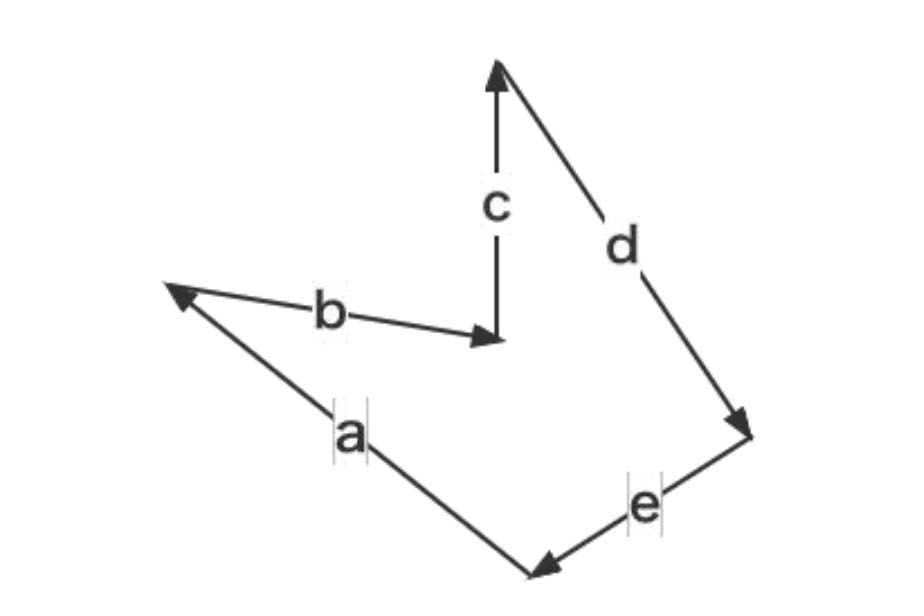
\includegraphics{bsp.jpg}
    \caption{problem}
\end{figure}

\begin{solution}
    其中 d 被 b 切割为 $\text{d}_1$ 和 $\text{d}_2$,如图 \ref{fig:bsp2} 所示,建立后的 BSP 树如图 \ref{fig:bsp} 所示。
    \begin{figure}[h]
        \centering
        \begin{minipage}[b]{.4\textwidth}
            \centering
            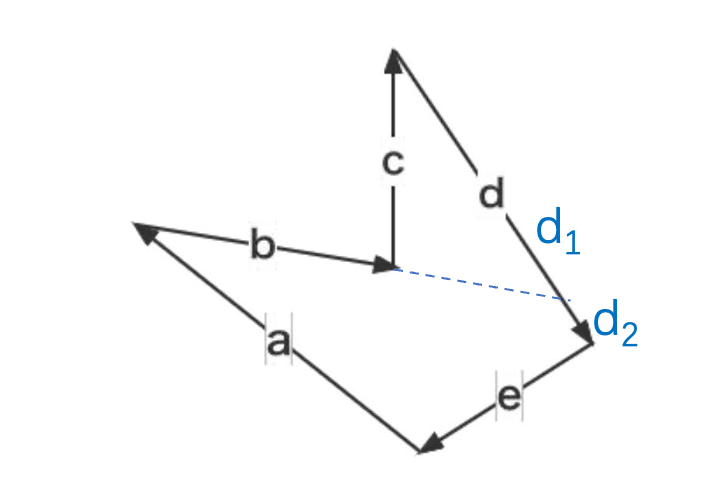
\includegraphics{bsp2.png}
            \caption{切割后的边}
            \label{fig:bsp2}
        \end{minipage}
        \begin{minipage}[b]{.4\textwidth}
            \begin{forest}
                [a[b[$\text{d}_2$[e[in][out]][out]][c[$\text{d}_1$[in][out]][out]]][out]]
            \end{forest}
            \caption{BSP 树}
            \label{fig:bsp}
        \end{minipage}
    \end{figure}
\end{solution}

\end{document}